\section{Our solution - better heading}
The system we have designed consists of two parts,
one being a input device
and the other being an application able to recognize the patterns from the device and forward predefined commands.

\subsection{Building the input device}
Our motion tracking device has been built in such a fashion that it resembles a wrist watch.
This form factor makes it rather compact.
Additionally alot of people wear watches on a daily basis which makes it recognizable and barely noticeable for people.

The specific device contains a list of components, the most important are 6DoF Sensor, Bluetooth and Arduino microcontroller.

\textbf{6DoF Sensor:}\\
This is the heart of the device. It contains an accelerometer and a gyroscope. This means we can measure movement and rotation of the wrist of anyone wearing the device.

\textbf{Arduino Pro Mini:}\\
This is the brain of the device, it handles all communication between the 6DoF chip and forwards the data over bluetooth to any consumers of the data.

The others are not that important to spend alot of time on, they provide means of communicating, charging and toggling the device on and off.

\begin{figure}[!h]
\centering
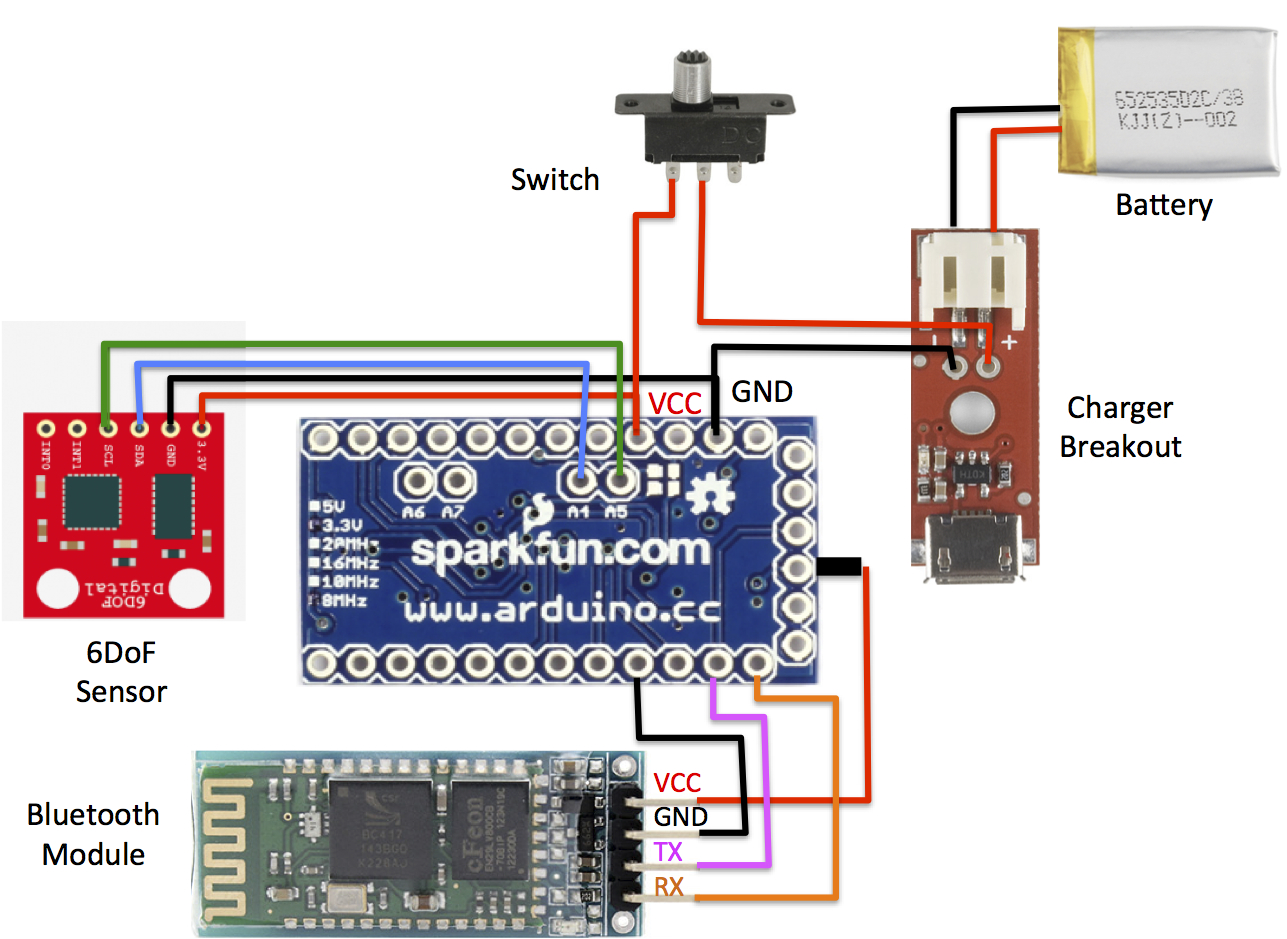
\includegraphics[width=0.9\columnwidth]{img/device_schematic}
\caption{This schematic shows the curcuitry on the device.}
\label{fig:figure1}
\end{figure}

\subsection{Big Data, slightly larger challenge}
Since the input device we have built is quite lightweight, data processing needs to be done elsewhere.
This provided us with the challenge of transfering data from one bluetooth capable device to another.
To 

\subsubsection{Raw Data and purifying}


\subsubsection{Pattern Recognition}